\documentclass[tikz,border=4pt]{standalone}
\usepackage{tikz}
\usetikzlibrary{positioning,arrows.meta,shapes.geometric,shapes.misc,decorations.pathmorphing,matrix}

\begin{document}
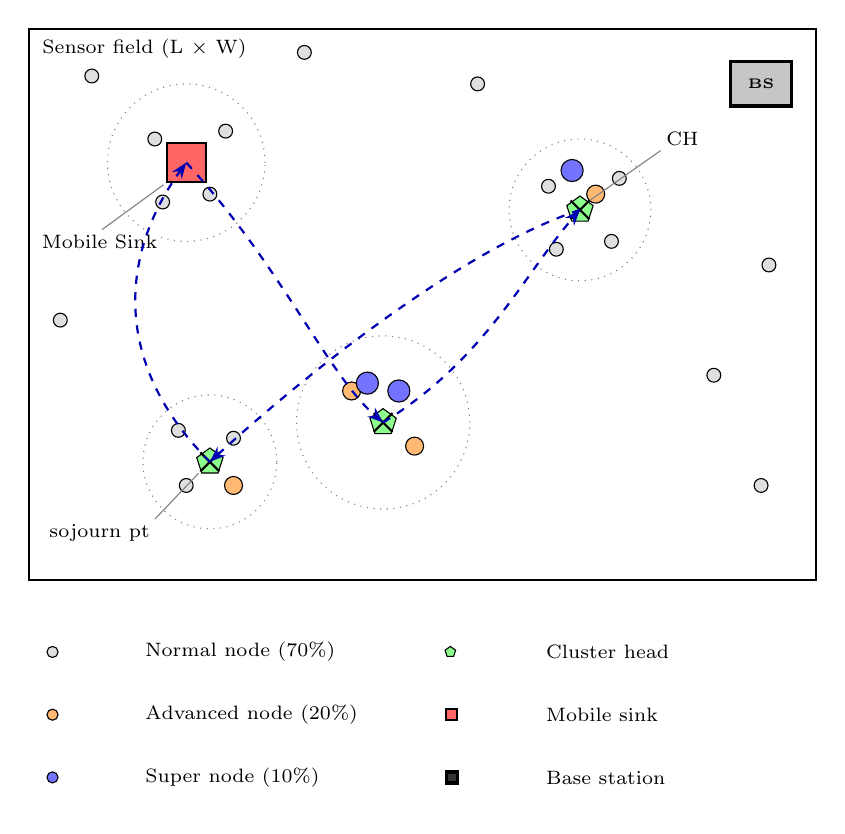
\begin{tikzpicture}[
    % In-field marker styles (real visual scale, distinguishable at map size)
    normalnode/.style={circle, draw, fill=gray!25, minimum size=5pt, inner sep=0pt},
    advnode/.style={circle, draw, fill=orange!55, minimum size=6.5pt, inner sep=0pt},
    supernode/.style={circle, draw, fill=blue!55, minimum size=8pt, inner sep=0pt},
    ch/.style={regular polygon, regular polygon sides=5, draw, fill=green!45, minimum size=10pt, inner sep=0pt},
    sink/.style={rectangle, draw, thick, fill=red!60, minimum size=14pt, inner sep=1pt},
    bs/.style={rectangle, draw, very thick, fill=gray!45, text=black, minimum width=22pt, minimum height=16pt, font=\tiny\bfseries},
    rp/.style={draw, cross out, thick, minimum size=6pt, inner sep=0pt},
    traj/.style={thick, blue!70!black, dashed, -{Stealth[length=2mm]}},
    covrange/.style={draw, dotted, gray},
    leader/.style={draw, gray, thin, shorten >=1pt, shorten <=1pt},
    % Legend swatch styles: every marker forced to the SAME ~4pt bounding box,
    % independent of its in-field visual scale above -- these are swatches,
    % not scale models, so sink/BS must not overrun their legend row.
    legnormalnode/.style={circle, draw, fill=gray!25, minimum size=4pt, inner sep=0pt},
    legadvnode/.style={circle, draw, fill=orange!55, minimum size=4pt, inner sep=0pt},
    legsupernode/.style={circle, draw, fill=blue!55, minimum size=4pt, inner sep=0pt},
    legch/.style={regular polygon, regular polygon sides=5, draw, fill=green!45, minimum size=4pt, inner sep=0pt},
    legsink/.style={rectangle, draw, thick, fill=red!60, minimum size=4pt, inner sep=0pt},
    legbs/.style={rectangle, draw, very thick, fill=black!80, minimum size=4pt, inner sep=0pt}
]

% Sensor field boundary
\draw[thick] (0,0) rectangle (10,7);
\node[anchor=north west, font=\scriptsize] at (0.05,7) {Sensor field (L $\times$ W)};

% Base station
\node[bs] (bs) at (9.3,6.3) {BS};

% Cluster head coverage ranges (dotted) + members
\foreach \cx/\cy/\r in {2/5.3/1.0, 4.5/2/1.1, 7/4.7/0.9, 2.3/1.5/0.85} {
  \draw[covrange] (\cx,\cy) circle (\r);
}

% Cluster heads
\node[ch] (ch1) at (2,5.3) {};
\node[ch] (ch2) at (4.5,2) {};
\node[ch] (ch3) at (7,4.7) {};
\node[ch] (ch4) at (2.3,1.5) {};

% Member sensor nodes (normal / advanced / super, scattered near each CH)
\foreach \x/\y in {1.6/5.6, 2.3/4.9, 1.7/4.8, 2.5/5.7} \node[normalnode] at (\x,\y) {};
\foreach \x/\y in {4.1/2.4, 4.9/1.7} \node[advnode] at (\x,\y) {};
\node[supernode] at (4.7,2.4) {};
\node[supernode] at (4.3,2.5) {};

\foreach \x/\y in {6.6/5.0, 7.4/4.3, 6.7/4.2, 7.5/5.1} \node[normalnode] at (\x,\y) {};
\foreach \x/\y in {7.2/4.9} \node[advnode] at (\x,\y) {};
\node[supernode] at (6.9,5.2) {};

\foreach \x/\y in {2.0/1.2, 2.6/1.8, 1.9/1.9} \node[normalnode] at (\x,\y) {};
\node[advnode] at (2.6,1.2) {};

% scattered background nodes (not yet clustered / periphery)
\foreach \x/\y in {0.6/0.6, 0.8/6.4, 9.3/1.2, 8.7/2.6, 5.7/6.3, 3.5/6.7, 0.4/3.3, 9.4/4.0} \node[normalnode] at (\x,\y) {};

% CH label: placed clear of ch3's own coverage circle and the super-node
% member above it, with a short leader line back to the marker. Drawn after
% all member nodes so it paints on top, not behind them.
\node[font=\scriptsize, fill=white, inner sep=1pt] (chlabel) at (8.3,5.6) {CH};
\draw[leader] (chlabel.south west) -- (ch3.north east);

% Mobile sink trajectory with rendezvous/sojourn points
\node[rp] (rp1) at (4.5,2) {};
\node[rp] (rp2) at (7,4.7) {};
\node[rp] (rp3) at (2.3,1.5) {};
\node[sink] (s1) at (2,5.3) {};
\node[font=\scriptsize, fill=white, inner sep=1pt] (sinklabel) at (0.9,4.3) {Mobile Sink};
\draw[leader] (sinklabel.north) -- (s1.south west);

\draw[traj] (2,5.3) .. controls (3.2,4.0) and (3.8,2.6) .. (4.5,2);
\draw[traj] (4.5,2) .. controls (5.8,2.8) and (6.3,3.9) .. (7,4.7);
\draw[traj] (7,4.7) .. controls (5.5,4.2) and (3.5,2.6) .. (2.3,1.5);
\draw[traj] (2.3,1.5) .. controls (1.0,2.8) and (1.2,4.2) .. (2,5.3);

% sojourn-pt label: placed below-left of rp3, clear of ch4's coverage circle
\node[font=\scriptsize, fill=white, inner sep=1pt] (sojournlabel) at (0.9,0.6) {sojourn pt};
\draw[leader] (sojournlabel.north east) -- (rp3.south west);

% Legend: fixed-grid matrix, uniform swatch scale, explicit row/column sep,
% placed with a clear gap below the field boundary. Left-aligned labels,
% markers anchored so every row's baseline lines up regardless of marker shape.
\matrix[
    anchor=north west,
    row sep=9pt,
    column sep={5pt,18pt,5pt},
    nodes={anchor=west, font=\scriptsize}
] at (0.1,-0.55) {
  \node[legnormalnode]{}; & \node{Normal node (70\%)}; & \node[legch]{};   & \node{Cluster head};  \\
  \node[legadvnode]{};    & \node{Advanced node (20\%)}; & \node[legsink]{}; & \node{Mobile sink};   \\
  \node[legsupernode]{};  & \node{Super node (10\%)};   & \node[legbs]{};   & \node{Base station};  \\
};

\end{tikzpicture}
\end{document}
